\section{图划分算法}

图数据划分问题是经典的NP(Non-deterministic Polynomial)完全问题,通常很难在有限的时间内找到图划分的最优解。
尽管其是难解问题,从20世纪90年代初期至今,国内外研究者不断对图划分及其相关问题进行深入研究,提出了许多性能较好的图划分算法。
现主要有随机划分法、谱方法、启发式方法、多层划分算法等。

\subsection{随机划分}

散列划分是最经典的随机图划分算法之一。
每个节点都有唯一的ID,散列划分通过一个Hash函数计算各ID的哈希值,然后将哈希值相同的节点分配到相同的分区中。
散列划分的优势在于简单易实现,不需要额外的开销且划分均衡可控。
但这种方法的缺陷也是非常明显的,它没有考虑到图的内部结构,各节点会被随机地划分到各分区中,结果就是区间边会非常多,对后续的操作造成很大不便,并产生巨大的通信开销。

\subsubsection{哈希划分算法流程}

\begin{algorithm}[htbp]
\SetAlgoLined
\KwIn{a differentiable action-value function parameterization:
        $\hat{q} : \mathcal{S} \times \mathcal{A} \times \mathbb{R}^{d} \rightarrow \mathbb{R}$}
\KwIn{a policy $\pi$ (if estimating $q_{\pi}$ )}
Algorithm parameters: step size $\alpha \in (0,1]$, small $\epsilon > 0 $, a positive integer $n$\;
Initialize value-function weights $\mathbf{w} \in \mathbb{R}^{d}$ arbitrarily (e.g., $\mathbb{w} = 0$)
All store and access operations (for $S_t$, $A_t$, and $R_t$) can take their index mod $n + 1$ \;

\caption{Episodic semi-gradient $n$-step Sarsa for estimating $\hat{q} \approx q_* $ or $q_\pi$}
\end{algorithm}


\subsection{谱方法}

谱聚类(Spectral Clustering, SC)是一种基于图论的聚类方法,可以追溯到R.Leland和B.Hendrickson在1990年提出的谱方法。
谱聚类可以识别任意形状的样本空间,能够将带权无向图划分为两个或两个以上的最优子图,并保证结果收敛于全局最优解。

谱聚类利用样本数据的相似矩阵$L$(即拉普拉斯矩阵)进行特征分解,然后对特征向量进行聚类。
拉普拉斯矩阵反映了各节点间的连接信息,它可以通过图的度矩阵$D$和关联矩阵$A$求得:$L=D-A$
构造关联矩阵$A$需要计算样本两两之间的相似度值,这里一般使用高斯核函数来计算相似度。
度矩阵$D$是一个对角矩阵,对角元素$D_{ii}=deg⁡(i)$。

谱聚类使得子图内部尽量相似,子图间距离尽量较远。
常见谱聚类的最优目标函数有两种:

\begin{enumerate}
    \item 可以是\textbf{Min Cut},即割边最小分割——的Smallest cut
    \item 可以是\textbf{Normalized Cut},即分割规模差不多且割边最小的分割——Best cut
\end{enumerate}

$L$矩阵中的元素定义如下所示:

\begin{equation}
    L_{i j}=\left\{\begin{array}{cc}{1,} & {\text { if } e(i, j) \in E} \\ {-\operatorname{deg}(i),} & {\text { if } i=j} \\ {0,} & {\text { other }}\end{array}\right.
\end{equation}

基于图谱理论的划分方法的主要思想是:
如果图$G$是连通的,那么其第二小特征值(最小的是$0$)也就是Fiedler特征值将给出图的连通性的一个度量。
如果将每个节点按对应的Fiedler特征值进行排序,然后将排好的序列分成$k$个部分,每个部分的节点将构成一个分区,即可实现图划分。
然而从计算量上来看,Fiedler特征值的计算和排序都较为复杂。
谱方法能为许多不同类的问题提供较好的划分,但是谱方法的计算量非常大。

\subsubsection{谱聚类算法流程}

\begin{algorithm}[htbp]
\caption{谱聚类算法流程}
\SetAlgoLined
\KwIn{a differentiable action-value function parameterization:
        $\hat{q} : \mathcal{S} \times \mathcal{A} \times \mathbb{R}^{d} \rightarrow \mathbb{R}$}
\KwIn{a policy $\pi$ (if estimating $q_{\pi}$ )}

\end{algorithm}

\subsection{启发式算法}

启发式算法通常是在对图已经进行过划分的结果上对其进行优化调整的。
启发式算法的划分结果很大程度的依赖初始划分的结果,为获得较好划分结果,需要与能够产生好较优划分的算法结合。
为了提高算法的执行效率,启发式算法通常将随机划分的结果作为初始划分,然后通过一些局部优化的方法减少交叉边的数量以达到降低通信代价的优化目的。

W.Kernighan和S. Lin 提出了Kernighan-Lin算法[2],它是一种比较典型的基于启发式规则的求解策略。
KL算法是一种贪婪算法,其初始划分选取了递归二分法。
首先将图随机划分成两个子图且要求子图规模尽量一致即保证负载均衡,接着随机交换划分后两个子图的任意两个顶点并对其进行标记,依次选取未被标记的顶点进行交换,当所有标记过的顶点都经过交换之后,结束一轮迭代过程。
记录每次迭代的过程中记录的交叉边个数最少,即划分质量最优的时顶点的划分状态,并将这种状态作为下次迭代的初始化分,以此类推。
当下次迭代对划分质量无明显改善时,停止迭代。
KL算法流程图如下图所示。

\subsubsection{Kernighan-Lin算法流程}

\begin{algorithm}[htbp]
\caption{Kernighan-Lin算法流程}
\SetAlgoLined
\KwIn{未分区图数据$G(V,E)$}
\KwOut{已分区图数据$G'(V,E,P)$}
       
对$G(V,E)$进行随机划分,保证各个子图规模相等或者相似,得到图$G_r(V,E,P_{rand})$

\Repeat{$g_{max} \leq 0$}{

    compute D values for all a in A and b in B \\
    let $g_v$, $a_v$, and $b_v$ be empty lists \\
    \For{$n$ := $1$ to $|V|/2$}{
        find a from $A$ and $b$ from $B$, such that $g = D[a] + D[b] - 2*c(a, b)$ is maximal \\
        remove $a$ and $b$ from further consideration in this pass \\
        add $g$ to $gv$, $a$ to $av$, and $b$ to $bv$ \\
        update $D$ values for the elements of $A = A \ a$ and $B = B \ b$ \\
    }

    find $k$ which maximizes $g_{max}$, the sum of $gv[1],...,gv[k]$\\

    \If{$g_{max} > 0$}{
        Exchange av[1],av[2],...,av[k] with bv[1],bv[2],...,bv[k]
    }
}
\end{algorithm}

KL算法的时间复杂度为$O(TNN)$ ,其中$n$为节点数,$t$为迭代次数。
所以当图的数据很大时,执行时间过长,因此不适用于大规模图。
此外,KL算法是初始解敏感的算法,即产生一个较好初始社区的条件是事先得知社区的个数或平均规模,若初始解较差,则会造成收敛速度缓慢,最终解较差。
由于现实世界中的社区无法事先预知,故KL算法的实用价值不大。

\subsection{多层划分算法}

\begin{figure}[htbp]
    \centering
    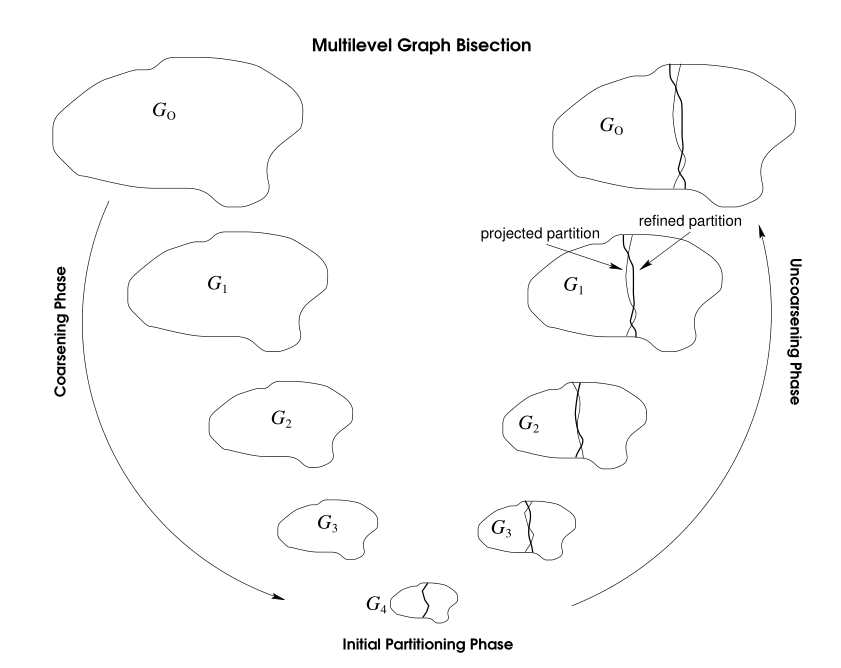
\includegraphics[width=0.75\linewidth]{figure/metis.png}
    \caption{}
    \label{}
\end{figure}

为了处理规模较大的图,文献[3]提出了多层的图划分框架METIS。
多层划分算法包括三个阶段:粗糙化 (coarsening) 阶段、初始划分、细化阶段(uncoarsening)。
第一阶段通过粗糙化技术将大图$G=(V,E)$约化为可接受的小图;
第二阶段将第一阶段获得的小图进行随机划分,并进行优化;
第三阶段通过细化技术以及优化技术将小图的划分还原为原图的划分。
该算法广泛地应用在各类大图的划分,对于百万规模以内的图,通常具有较好的实际效果。

\subsubsection{Metis算法流程}

\begin{algorithm}[htbp]
\caption{Metis算法流程}
\SetAlgoLined
\KwIn{未分区图数据$G_o(V_o,E_o)$}
\KwIn{分区数量$k$}
\KwOut{已分区图数据$G'(V,E)$}

\uIf{$n_t$足够小}{
    直接在图$G_t=(V_t,E_t)$上进行划分,得到对应的划分模式$P_t$ \\
    返回$P_t$ \\
}
\Else{
    粗化图$G_i$,得到一个规模较小的相似图$G_{i+1}$ \\
    迭代函数$P_{i+1}=METIS(G_{i+1})$,以找到一系列的粗化图,直到图的规模足够小,即找到图$G_t$\\
}

$i = t$; 	//用以记录细化阶段的层

\Repeat{$i==0$}{
$G_(i-1)=recover(G_i,P_i)$ 		//划分模式的投射 \\
$P_(i-1)*=refine(G_(i-1),P_(i-1))$ 	//改善划分质量\\ 
$i = i-1$ \\
}

\end{algorithm}

\subsubsection{粗化阶段}

在粗化阶段,一些联系较强的部分节点会聚集形成一个局部整体,这个局部整体会以一个带节点权重的超级节点 (Super node) 的形式呈现出来,而构成该局部整体的节点以及它们之间的边会暂时的从图中隐藏掉,同时对外只呈现出一个权重节点。为了得到这些局部整体,需要将部分图顶点进行融合。顶点融合的最终目的是为了减小原始图的规模,因此顶点的匹配应该最大化。最大匹配的定义如下:如果一个匹配在不使两条边指向同一个顶点的情况下无法再增加新的边,这个匹配叫做图的最大匹配。(由于匹配的计算方法不同,最大匹配的结果可能会有差异)。

经常用到的寻找匹配的策略主要有两种:随机策略(Random Matching,RM) 和权重边策略(Heavy edge matching,HEM)。

\paragraph{随机策略}
随机策略算法顾名思义,即随机选取边来组成一个匹配,其时间复杂度为$O(m)$。
用随机算法可以快速有效地生成一个匹配随即最大匹配算法,按照如下步骤工作:
先按照随机的顺序遍历原始图中所有的顶点,如果一个顶点u还没有被匹配,算法会随机地选择其尚未匹配的相邻顶点。
如果存在这样的相邻顶点$v$,就将边$(u,v)$加入匹配中。
如果己经不存在未配的相邻顶点,则顶点$u$标记为未匹配顶点。
这种策略虽然可以有效地找出一个极大匹配,但却没有考虑边和节点的权重值等信息。

\paragraph{权重边策略}
权重边匹配即在用重边策略寻找匹配时要尽可能地选择边权重值最大的边,是一种简单有效的求取最大匹配的方法。
在粗化过程中生成的各图的节点数在不断减少,但各图中节点的权重之和始终保持不变,但各图中的边权重之和却在持续减小。
对于粗化过程中生成的两个连续的图$G_i=(V_i,E_i)$和$G_(i+!)=(V_(i+1),E_(i+1))$以及从$G_i$生成$G_(i+1)$过程中的一个匹配$M_i \in E_i$。
如果A是边的集合,定义$W(A)$为$A$中边的权值的总和。
显然可以得到:$W(E_(i+1) )=W(E_i )-W(M_i )$
其中,$W(E_i)$和$W(E_(i+1))$分别表示图$G_i$和$G_(i+1)$中的边的权重值之和,而$W(M_i)$则表示匹配$M_i$中的所有边的权重值之和。

由此可见,粗化后的图中的边权重之和与粗化过程中的匹配有很大的关系。如果匹配中的边权重之和越大,则粗化后的图中边权重之和越小,反之亦然。所以,HEM使得匹配中的边权重之和最大化,即在每一次的粗化过程中尽可能多的减少边权重,从而在粗化过程结束时得到的图中的边权重之和最小。

\subsubsection{初始划分阶段}

Metis第二步是对粗化后的图进行k路划分。
对粗化图$G_m=(V_m,E_m)$计算划分$P_m$使得划分后的每部分大致均勾地含有原图的$|V|/k$个顶点。

一种产生$k$路初始划分的办法就是不断地对原图进行粗化操作,直到粗化图只剩下$k$个顶点。
这个含有$k$个顶点的粗化图可以作为原始图的$k$路初始划分。
在这个过程中会产生两个问题:
\begin{enumerate}
    \item 对于很多图来说,在进行了几次粗化之后,每一次的粗化过程所能减少的图的规模过小,因此粗化耗费的资源会很大。
    \item 即使将原图粗化到了仅剩个顶点,这些顶点的权值也极有可能差异很大,最终导致初始划分的平衡度大大降低。
\end{enumerate}

多级划分算法是算法的基本思想,就是在进行了顶点融合算法之后,原图的规模已经减小到了比较容易处理的地步。
经过顶点粗化的处理以后,顶点数和边数大大减少的新图将更有利于初始划分的进行。
在多级划分中,初始划分就是现将图进行二路划分,并在划分的同时考虑负载的平衡。
初始划分常用的算法是几何划分和谱划分等。
由于概化图规模一般较小,执行以上算法通常耗时很少。

\subsubsection{细化阶段}

如前所述,细化阶段是粗化阶段的反过程,其实就是还原过程。
在细化过程中,在粗化过程中被隐藏的边和节点将会逐步重新呈现出来,

在这个步骤中,粗化图的划分,会通过回溯每一级的粗化图$G_m$的划分$P_m$还原成原图。
虽然$P_{i+1}$是$G_{i+1}$的局部最小划分,但是细化后的划分$P_i$可能不再是$G_i$的局部最小划分。
由于$G_i$更加精细,所以会有更大的自由度优化$P_i$以减少边割。
因此,仍然可以使用局部细化启发式算法例如KL算法来优化划分$G_{i+1}$的划分。
每进行一次细化,算法会对细化后的划分使用优化算法。
划分优化算法的最基本思想是在划分后的两个部分中选择两个顶点集合进行互换,如果得到的新划分有更小的边割,则采用新的划分。
